\chapter[RMQ]{Range Minimum Query}
\writer{Felix Lauenroth \& Michael Mardaus}

\section{Einleitung}

Im Folgenden besch�ftigen wir uns mit dem $Range Minimum Query (RMQ)$ Algroithmus und dem Skyline Problem. In Kapitel 1 behandeln wir den $RMQ$ und Kapitel 2 handelt vom Skyline Problem. Kommen wir zun�chst zur Definition der $ RMQ $. Gesucht wird die Indexposition des kleinsten Wertes innerhalb einem gegebenem Intervall [l, r] oder mathematisch Ausgedr�ckt:

\[\text{RMQ}_{A}(\ell,r) = \text{arg} \ \min_{\ell \leq k \leq r } A[k] \]

\section{Naive Ans�tze}
\subsection{Durch iterieren}

Zun�chst beschreiben wir eine auf den ersten Blick einfach aussehende Methode. Wir iterieren sequenziell durch das gegebene Intervall und speichern dabei die Indexposition des Minimums. Dies schaffen wir offensichtlich in $\Oh(n)$ \footnote{\label{foot:1} $n$ beschreibt die L�nge des Intervalls}. Wie auf den ersten Blick erkennbar ist variiert die Laufzeit mit der L�nge des gegebenen Intervalls. Auch bei mehrfach Ausf�hrung der Abfrage verschlechtert sich die Laufzeit um den erheblichen Faktor $m$\footnote{\label{foot:2} $m$ beschreibt die Anzahl der Abfragen}, welches zu einer Laufzeit von $\Oh(n\cdot m)$ bei $m$ Abfragen f�hrt. Doch diese Methode hat einen erheblichen Vorteil. Sie funktioniert in-place, das hei�t sie ben�tigt nur eine konstante Menge an Speicher. Denn das durch-iterieren findet in der Eingabeliste statt und ansonsten wird nur Speicherplatz f�r die Indexposition ben�tigt.

\subsection{Preprocessing}

Kommen wir nun zur Anschauung des Preprocessings. Hierbei erstellt man sich zun�chst eine $n\times n$ Matrix $M$, in der man alle Kombinationsm�glichkeiten des Intervalls vorberechnet.

\subsection{Preprocessing mit dynamischer Programmierung}

\section{Effiziente Algorithmen}
\subsection{$\sqrt n $ Teile Algorithmus}

\subsection{Sparse Table}
Als n�chstes er�rtern wir den Sparse Table Algorithmus ($STA$) welcher auf Preprocessing zur�ck greift. Der $STA$ besteht im Wesentlichen aus zwei Phasen. In Phase 1 wird zun�chst die Zweierpotenz errechnet, welche mindestens die H�lfte der Eingabeliste �berdeckt. Denn Exponenten\footnote{\label{sparse:1}zur Basis 2} dieser Zweierpotenz nennen wir im Folgenden $n$. Nun wird ein Matrix $A[][]$ mit $pos$ Spalten und $n$ Zeilen angelegt. Der Zeilenindex entspricht hierbei dem Exponenten einer Zweierpotenz\footnote{\label{sparse:2} 
\begin{tabular}{l}
$A[0][0]\equiv 2^0$ \\ 
$A[0][1]\equiv 2^1$ \\
\end{tabular}
}. Anschlie�end wird 
Anhand 

die Indexposition des Minimus, der entsprechenden L�nge, in der Matrix $A[][]$ gespeichert (Abb. \ref{sparse_1}).
\begin{figure}[h]
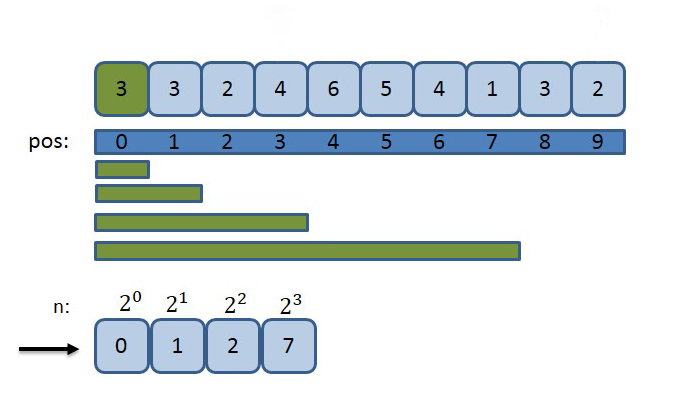
\includegraphics[width=7cm]{picture/sparse_1.png}
\caption{Phase 1}
\label{sparse_1}
\end{figure}
Dies geschieht f�r jeden Eintrag der Liste. 
Nachdem Phase 1 beendet ist, habe wir das Preprocessing  

\chapter{Skyline}

\section{Problemstellung}

\section{Anhang}
